% ===== Section 2: Come on, feel the noise (hearing and touch, ~14 min), then the break =====
\topicopener{ear}{Լսողություն ու հպում}{Արի՛, զգա աղմուկը}{Ինչով են իրար նման լսողությունն ու հպումը}{happy}

\begin{frame}{Ականջի փայտիկի սկզբունքը}
  \begin{columns}[T]
    \begin{column}{0.52\textwidth}
      \begin{bookquote}
        Նկատե՞լ ես, թե որքան հաճելի է ականջը փայտիկով մաքրելը։ Այո՞։ Դա այս թեմայի հետ կապ չունի, ես պարզապես սկզբունքն եմ հաստատում։
      \end{bookquote}
      \onslide<2->{%
      Ե՞րբ է որևէ ձայն քեզ «կպչուն» թվացել, կամ հպումը՝ «բարձր»։ Երբեք, չէ՞։\par\smallskip
      \textbf{Իրականում՝ սխալվում ես։}}
    \end{column}
    \begin{column}{0.44\textwidth}
      \onslide<3->{%
      \begin{poll}
        \emoji{speaker}\ Բարձրացրու ձեռքդ, եթե համերգին կամ մեքենայում \textbf{բասը զգացել ես կրծքիդ մեջ}։
      \end{poll}}
      \vspace{1mm}
      \onslide<4->{%
      \begin{card}[colback=lavender!40!cardwhite]
        Բավականաչափ ուժեղ կամ ցածր ձայնը \textbf{ֆիզիկական} է դառնում. ատամների պլոմբներն են դղրդում։
      \end{card}}
    \end{column}
  \end{columns}
\end{frame}

\begin{frame}{Երկու զույգ զգայարան}
  \begin{columns}[T]
    \begin{column}{0.47\textwidth}
      \begin{card}[colback=peach!40!cardwhite]
        \emoji[1.3em]{nose}\emoji[1.3em]{tongue}\ {\blackfont Քիմիական}\par\smallskip
        Հոտ ու համ։ Արձագանքում են որոշակի \textbf{քիմիական նյութերի}՝ մրգահյութ, դոնդողե արջուկներ։
      \end{card}
    \end{column}
    \begin{column}{0.47\textwidth}
      \onslide<2->{%
      \begin{card}[colback=mint!40!cardwhite]
        \emoji[1.3em]{ear}\emoji[1.3em]{hand}\ {\blackfont Մեխանիկական}\par\smallskip
        Լսողություն ու հպում։ Արձագանքում են \textbf{ճնշմանը} կամ ֆիզիկական ուժին։
      \end{card}}
    \end{column}
  \end{columns}
  \vspace{3mm}
  \onslide<3->{%
  \begin{card}[colback=butter!40!cream]
    \centering\emoji{speaker}\ Ձայնը \textbf{օդի տատանում} է։ Այն հասնում է ականջին ու տատանում է թմբկաթաղանթը։ Այսինքն՝ ձայնը «դիպչում» է քեզ։
  \end{card}}
\end{frame}

\begin{frame}{Ձայնի ճանապարհը}
  \centering
  % The route of a sound: air waves -> ear canal -> eardrum -> three tiny bones -> cochlea (hair cells)
% -> 8th cranial nerve -> auditory cortex. Captions alternate above/below. Reveals in 5 steps.
\begin{tikzpicture}[
    capt/.style={font=\scriptsize, text=plum, align=center, text width=2.6cm},
  ]
  \path[use as bounding box] (-6.9,-1.4) rectangle (6.9,1.5);
  % sound waves and the ear canal
  \foreach \r in {0.3,0.55,0.8}{\draw[amBlue, line width=1.1pt] (-6.9,0) ++(-28:\r) arc (-28:28:\r);}
  \filldraw[fill=peach!50!cardwhite, draw=plum, line width=0.9pt]
    (-5.9,1.0) .. controls (-5.5,0.55) .. (-5.0,0.32) -- (-3.6,0.32) -- (-3.6,-0.32) -- (-5.0,-0.32)
    .. controls (-5.5,-0.55) .. (-5.9,-1.0);
  \node[capt, anchor=north] at (-4.7,-0.65) {օդի տատանումները\\ ականջի անցուղում};
  % eardrum
  \filldraw[fill=pinkdark, draw=plum, line width=0.6pt, visible on=<2->] (-3.5,0) ellipse (0.09 and 0.6);
  \node[capt, anchor=south, visible on=<2->] at (-3.5,0.75) {\textbf{թմբկաթաղանթ}\\ բարակ թաղանթ};
  % the three tiny bones
  \begin{scope}[visible on=<3->]
    \filldraw[fill=butter, draw=plum, line width=0.7pt, rotate around={-35:(-3.0,0.2)}] (-3.0,0.2) ellipse (0.36 and 0.14);
    \filldraw[fill=butter, draw=plum, line width=0.7pt] (-2.45,0.28) ellipse (0.24 and 0.2);
    \filldraw[fill=butter, draw=plum, line width=0.7pt] (-2.15,0.13) -- (-1.7,0.13) -- (-1.7,-0.22) -- (-1.8,-0.22)
      -- (-1.8,0.03) -- (-2.05,0.03) -- (-2.05,-0.22) -- (-2.15,-0.22) -- cycle;
    \node[capt, anchor=north] at (-2.35,-0.65) {\textbf{3 ոսկրիկ}\\ մուրճ, սալ, ասպանդակ};
  \end{scope}
  % cochlea
  \begin{scope}[visible on=<4->]
    \draw[plum, line width=0.8pt] (-1.7,0.0) -- (-0.45,0.0);
    \draw[plum, line width=4.2pt, domain=0:11, samples=140, variable=\t]
      plot ({0.4+(0.08+0.075*\t)*cos(\t r)}, {0.05+(0.08+0.075*\t)*sin(\t r)});
    \draw[lavender, line width=2.6pt, domain=0:11, samples=140, variable=\t]
      plot ({0.4+(0.08+0.075*\t)*cos(\t r)}, {0.05+(0.08+0.075*\t)*sin(\t r)});
    \node[capt, anchor=south, text width=2.6cm] at (0.4,0.95) {\textbf{խխունջ}, մազիկավոր\\ բջիջներ (hair cells)};
  \end{scope}
  % nerve and cortex
  \begin{scope}[visible on=<5->]
    \draw[amOrange!85!black, line width=1.6pt, decorate, decoration={snake, amplitude=0.6mm, segment length=3mm}]
      (1.4,0.05) -- (3.9,0.05);
    \node[capt, anchor=north] at (2.65,-0.65) {\textbf{VIII նյարդ}\\ (vestibulocochlear)};
    \node at (4.85,0.1) {\bigemoji[0.9cm]{brain}};
    \node[capt, anchor=south, text width=2.6cm] at (4.85,0.75) {\textbf{լսողական կեղև}\\ քունքային բիլթ};
  \end{scope}
\end{tikzpicture}
\par\medskip
  \onslide<6->{%
  \begin{scienceupdate}[width=0.92\textwidth]
    Գրքում՝ «թմբկաթաղանթը կազմված է երեք փոքրիկ ոսկրից»։ Իրականում այն \textbf{բարակ թաղանթ} է, իսկ ոսկրիկները նրա հետևում են՝ միջին ականջում։
  \end{scienceupdate}}
\end{frame}

\begin{frame}{Խխունջը՝ հաճախականությունների քարտեզ}
  \centering
  % The cochlea unrolled: a frequency map. High pitches peak near the start (base), low pitches near the
% end (apex). Tick positions are schematic (roughly logarithmic), the 20-20,000 Hz range is from the book.
% Reveals: 2 = high-pitch wave, 3 = low-pitch wave (use inside a frame).
\begin{tikzpicture}[x=1cm, y=1cm]
  \path[use as bounding box] (-0.6,-1.6) rectangle (11.4,1.6);
  % the unrolled tube
  \shade[left color=amRed!55!cardwhite, right color=amBlue!45!cardwhite, rounded corners=3mm]
    (0,-0.45) -- (10.6,-0.25) -- (10.6,0.25) -- (0,0.45) -- cycle;
  \draw[plum, line width=1pt, rounded corners=3mm] (0,-0.45) -- (10.6,-0.25) -- (10.6,0.25) -- (0,0.45) -- cycle;
  \foreach \f/\x in {20\,000/0.35, 2000/3.6, 200/6.95, 20/10.25}{
    \draw[plum, line width=0.8pt] (\x,-0.5) -- (\x,-0.68);
    \node[font=\blackfont\scriptsize, text=plum, below] at (\x,-0.66) {\f\ Հց};}
  \node[font=\scriptsize, text=plum, anchor=north west] at (-0.1,-1.15) {\textbf{սկիզբ}};
  \node[font=\scriptsize, text=plum, anchor=north east] at (10.7,-1.15) {\textbf{վերջ}};
  \node[font=\scriptsize, text=plum!75!cream] at (5.3,-1.45) {մարդը լսում է մոտ 20-ից 20\,000 Հց};
  % high pitch: peaks near the start
  \begin{scope}[visible on=<2->]
    \draw[amRed, line width=1.2pt, domain=0.15:4.0, samples=220, variable=\t]
      plot (\t, {0.32*exp(-((\t-1.1)^2)/0.6)*sin(\t*1600)});
    \node[anchor=south west, font=\footnotesize, text=plum, align=left] at (0.0,0.62)
      {\emoji{balloon}\ \textbf{բարձր ձայներ}\\ «հելիում շնչած հուզված փոքրիկ»};
  \end{scope}
  % low pitch: peaks near the end
  \begin{scope}[visible on=<3->]
    \draw[amBlue, line width=1.2pt, domain=5.5:10.5, samples=160, variable=\t]
      plot (\t, {0.26*exp(-((\t-9.0)^2)/1.4)*sin(\t*260)});
    \node[anchor=south east, font=\footnotesize, text=plum, align=right] at (10.7,0.62)
      {\textbf{ցածր ձայներ} \emoji{musical}\\ «Բարրի Ուայթ երգող կետ»};
  \end{scope}
\end{tikzpicture}
\par\vspace{-1mm}
  \begin{columns}[T]
    \begin{column}{0.47\textwidth}
      \onslide<4->{\small Խխունջը (cochlea) պարույր, հեղուկով լի խողովակ է։ \textbf{Հաճախականությունից} է կախված, թե տատանումը որքան հեռու կգնա։}
    \end{column}
    \begin{column}{0.47\textwidth}
      \onslide<5->{\small Ուղեղը գիտի, թե \textbf{որ մասից} է ազդանշանը եկել, ու այդպես է «լսում» ձայնի բարձրությունը։}
    \end{column}
  \end{columns}
\end{frame}

\begin{frame}{Երբ լսողությունը սխալվում է}
  \begin{columns}[T]
    \begin{column}{0.31\textwidth}
      \begin{card}[colback=butter!45!cardwhite]
        \emoji[1.3em]{construction}\ {\blackfont Մեխանիկա}\par\smallskip
        Անընդհատ թափահարվող նուրբ համակարգ։ Հեղուկ, ականջի ծծումբ, վնասվածք։ Տարիքի հետ հյուսվածքները կարծրանում են. չկա տատանում, չկա ձայն։
      \end{card}
    \end{column}
    \begin{column}{0.31\textwidth}
      \onslide<2->{%
      \begin{card}[colback=peach!40!cardwhite]
        \emoji[1.3em]{bell}\ {\blackfont Ականջի «զնգոց»}\par\smallskip
        Ձայներ առանց դրսի աղբյուրի՝ ականջի խնդիրներից (endaural phenomena), օրինակ՝ \textbf{տինիտուս}։
      \end{card}}
    \end{column}
    \begin{column}{0.31\textwidth}
      \onslide<3->{%
      \begin{card}[colback=lavender!40!cardwhite]
        \emoji[1.3em]{brain}\ {\blackfont Լսողական հալյուցինացիաներ}\par\smallskip
        Ուղեղի «վերին» մասերից՝ ձայներ լսել, «երաժշտական ականջի համախտանիշ», «պայթող գլխի համախտանիշ»։
      \end{card}}
    \end{column}
  \end{columns}
  \vspace{2mm}
  \onslide<4->{\centering\small Բըրնեթ՝ «պայթող գլուխը» «ավելի վատ է հնչում, քան կա»։\par}
\end{frame}

\begin{frame}{Հպումը մեկ զգայարան չէ}
  \begin{columns}[T]
    \begin{column}{0.55\textwidth}
      \begin{tikzpicture}
        \foreach \x/\e/\t/\c in {0/hand/ճնշում/cardwhite, 1.45/phone/թրթռոց/mint!40!cardwhite,
            2.9/thermometer/ջերմ/peach!45!cardwhite, 4.35/muscle/ձգում/butter!60!cardwhite,
            5.8/bandage/ցավ/brainpink!35!cardwhite}{
          \node[wtile=\c, minimum width=1.3cm] at (\x,0) {\emoji[1.5em]{\e}\\[1pt] \textbf{\t}};}
      \end{tikzpicture}\par\medskip
      \begin{itemize}
        \item Ամեն մեկն իր ընկալիչներն ունի։ Ցավը՝ նոցիցեպցիան (nociception), նույնպես
        \item<2-> Մաշկ $\rightarrow$ ողնուղեղ $\rightarrow$ \textbf{զգացողական կեղև} (somatosensory cortex) գագաթային բլթում
      \end{itemize}
    \end{column}
    \begin{column}{0.41\textwidth}
      \onslide<3->{%
      \begin{card}[colback=lavender!40!cardwhite]
        \emoji[1.3em]{brain}\ Ցավի ընկալիչներ գրեթե միայն \textbf{ուղեղը} չունի։ Այն ինքն է ցավը մշակում։
      \end{card}
      \begin{bookquote}
        Ուղեղի ցավ զգալը նման կլիներ սեփական համարիդ զանգելուն ու սպասելուն, որ ինչ-որ մեկը կպատասխանի։
      \end{bookquote}}
    \end{column}
  \end{columns}
\end{frame}

\begin{frame}{Մարմնի քարտեզը ուղեղում}
  \begin{columns}[c]
    \begin{column}{0.42\textwidth}
      \centering
      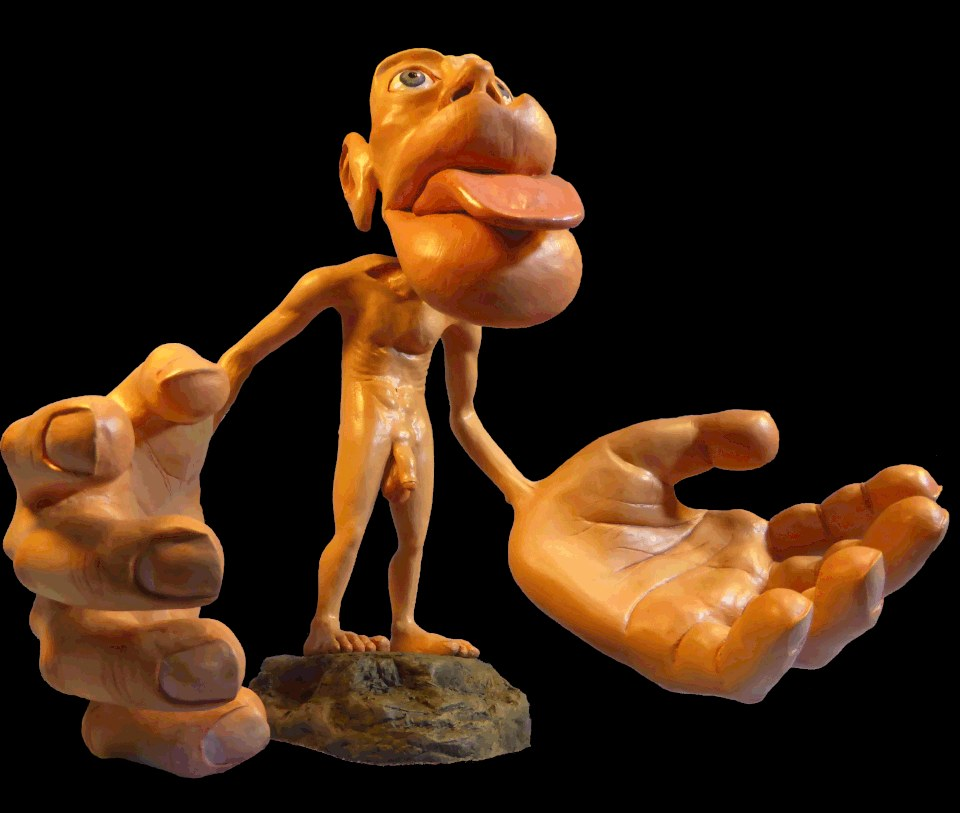
\includegraphics[height=5.0cm]{homunculus_model.jpg}\par
      {\scriptsize Զգացողական հոմունկուլուս (homunculus)}
    \end{column}
    \begin{column}{0.54\textwidth}
      \begin{itemize}
        \item Զգացողական կեղևը մարմնի \textbf{քարտեզ} է. ոտքի հատվածը ոտքի համար, ձեռքինը՝ ձեռքի
        \item<2-> Բայց չափերը \textbf{իրական չեն}. կուրծքն ու մեջքը փոքր տեղ ունեն, ձեռքերն ու շուրթերը՝ հսկայական
        \item<3-> Ներբանները շատ զգայուն չեն. այլապես ամեն քարի վրա ոտք դնելը տանջանք կլիներ
        \item<4-> «Սեռական օրգանները նույնպես զգայուն են, բայց եկեք չխորանանք» (Բըրնեթ)
      \end{itemize}
    \end{column}
  \end{columns}
\end{frame}

\begin{frame}{Երկու կետ, թե՞ մեկ}
  \begin{columns}[T]
    \begin{column}{0.45\textwidth}
      \begin{tryit}
        Երկու գրիչի ծայրերը պահիր \textbf{մոտ 1 սմ} հեռու ու դիպցրու \textbf{մատիդ ծայրին}, հետո՝ \textbf{նախաբազկին}։ Քանի՞ կետ ես զգում։
      \end{tryit}
      \onslide<3->{%
      \begin{card}[colback=butter!40!cream]
        \emoji{hand}\ Դրա համար են \textbf{Բրայլի} տառերը կետերից. մատի ծայրը սովորական տառեր չի «կարդա»։
      \end{card}}
    \end{column}
    \begin{column}{0.51\textwidth}
      \onslide<2->{%
      {\small\blackfont Ամենափոքր հեռավորությունը, որ երկու կետը զգացվում է որպես երկու, մմ}\par\medskip
      % Two-point discrimination: the smallest gap at which two touches feel like two (normal clinical ranges,
% Bickley & Szilagyi, Bates' Guide, 2007). Range bars on a 0-40 mm axis (use inside a frame).
\begin{tikzpicture}[x=0.1cm, y=1cm]
  \draw[plum, line width=0.8pt] (0,-0.35) -- (41,-0.35);
  \foreach \m in {0,10,20,30,40}{
    \draw[plum, line width=0.8pt] (\m,-0.35) -- (\m,-0.47);
    \node[font=\scriptsize, text=plum, below] at (\m,-0.45) {\m};}
  \foreach \y/\t/\a/\b in {2.4/շուրթեր/2/4, 1.65/մատի ծայր/2/8, 0.9/ափ/8/12, 0.15/{մեջք, սրունք}/30/40}{
    \node[font=\small, text=plum, anchor=east] at (-0.8,\y) {\t};
    \fill[amBlue, rounded corners=1mm] (\a,\y-0.2) rectangle (\b,\y+0.2);
    \node[font=\blackfont\scriptsize, text=plum, anchor=west] at (\b+0.6,\y) {\a-\b};}
\end{tikzpicture}
}
    \end{column}
  \end{columns}
  \onslide<2->{\source{Bickley \& Szilagyi, Bates' Guide, 2007}}
\end{frame}

\begin{frame}{Արիստոտելի իլյուզիա}
  \begin{columns}[c]
    \begin{column}{0.5\textwidth}
      \begin{tryit}
        \begin{enumerate}
          \item Խաչիր ցուցամատդ ու միջնամատդ
          \item \textbf{Փակիր աչքերդ}
          \item Խաչված մատների ծայրերով շոշափիր գնդիկը, մետաղադրամի եզրը կամ քթիդ ծայրը
        \end{enumerate}
        Քանի՞ առարկա ես զգում։
      \end{tryit}
    \end{column}
    \begin{column}{0.46\textwidth}
      \centering
      % Aristotle's illusion: with crossed fingers, one small ball touches the two "outer" sides of the
% fingertips, and the brain reports two balls. The thought bubble appears on slide 2 (use inside a frame).
\begin{tikzpicture}[scale=0.82]
  \path[use as bounding box] (-2.0,-2.3) rectangle (3.6,2.5);
  % palm
  \filldraw[fill=peach!70!cardwhite, draw=plum, line width=0.9pt, rounded corners=4mm] (-1.05,-2.25) rectangle (1.05,-1.05);
  % index finger (under), then middle finger (over), crossed
  \draw[plum, line width=0.56cm, line cap=round] (-0.42,-1.15) -- (0.5,1.05);
  \draw[peach!70!cardwhite, line width=0.42cm, line cap=round] (-0.42,-1.15) -- (0.5,1.05);
  \draw[plum, line width=0.56cm, line cap=round] (0.42,-1.15) -- (-0.5,1.05);
  \draw[peach!70!cardwhite, line width=0.42cm, line cap=round] (0.42,-1.15) -- (-0.5,1.05);
  % the ball between the crossed tips
  \shade[ball color=amBlue!70] (0,1.62) circle (0.3);
  \node[font=\blackfont\small, text=plum, anchor=east] at (-0.6,1.75) {1 գնդիկ};
  % what the brain reports
  \node[think, visible on=<2->, callout absolute pointer={(0.7,1.75)}, minimum width=2.4cm, minimum height=1.6cm]
    at (2.45,1.55) {\tikz{\shade[ball color=amBlue!70] (0,0) circle (0.2); \shade[ball color=amBlue!70] (0.55,0) circle (0.2);}\\[1mm] 2 գնդիկ};
\end{tikzpicture}
\par
      \onslide<3->{\raggedright\small Զգացողական կեղևը «չգիտի», որ մատները խաչված են, իսկ փակ աչքերը չեն կարող օգնել։\par}
    \end{column}
  \end{columns}
\end{frame}

\begin{frame}{Գեները կապում են լսողությունն ու հպումը}
  \begin{columns}[c]
    \begin{column}{0.56\textwidth}
      \begin{itemize}
        \item 2012. Ֆրենցելն (Frenzel) ու գործընկերները ցույց տվեցին, որ գեները ազդում են նաև \textbf{հպման զգայունության} վրա
        \item<2-> Ով շատ լավ է լսում, սովորաբար ավելի նուրբ հպում էլ ունի. ով վատ է լսում, հաճախ վատ է զգում նաև հպումը
        \item<3-> Գտան նաև մի մուտացված գեն, որը վնասում է \textbf{երկուսն էլ}
      \end{itemize}
    \end{column}
    \begin{column}{0.4\textwidth}
      \centering
      \bigemoji[1.2cm]{ear}\ {\Large $\leftrightarrow$}\ \bigemoji[1.2cm]{hand}\par\medskip
      \onslide<4->{%
      \begin{card}[colback=mint!35!cardwhite]
        Ուրեմն ռիթմը զգալը, գուցե, ավելի \textbf{բառացի} է, քան կարծում էինք \emoji{musical}
      \end{card}}
    \end{column}
  \end{columns}
  \source{Frenzel et al., PLOS Biology, 2012}
\end{frame}

\begin{frame}{Առաջին կեսը՝ մեկ էջում}
  \begin{columns}[T]
    \begin{column}{0.47\textwidth}
      \begin{card}\emoji{nose}\ {\blackfont Հոտ}\par Թերագնահատված է. 1 տրիլիո՞ն հոտ, ուղիղ կապ հիշողության ու զգացմունքների հետ\end{card}
      \begin{card}\emoji{tongue}\ {\blackfont Համ}\par Ամենաթույլը. մեծ մասը հոտն է, մնացածը՝ ակնկալիքը\end{card}
    \end{column}
    \begin{column}{0.47\textwidth}
      \begin{card}\emoji{ear}\ {\blackfont Լսողություն}\par Մեխանիկական. խխունջը հաճախականությունների քարտեզ է\end{card}
      \begin{card}\emoji{hand}\ {\blackfont Հպում}\par Ուղեղում մարմնի աղավաղված քարտեզ, ու այն էլ է խաբվում\end{card}
    \end{column}
  \end{columns}
  \vspace{1mm}
  \centering\small Ուղեղը սիրում է զգայարանները \textbf{զույգերով} խմբավորել, ավելի հաճախ, քան գործնական է։
\end{frame}

% ---------------------------------------------------------------- break
\begin{frame}[plain]
  \begin{tikzpicture}[remember picture, overlay]
    \fill[butter!60!cream] (current page.south west) rectangle (current page.north east);
    \node at ([yshift=8mm]current page.center) {\mascot[4cm]{sleepy}};
    \node[anchor=north, font=\titlefont\fontsize{30}{32}\selectfont, text=plum] at ([yshift=-17mm]current page.center) {Ընդմիջում};
    \node[anchor=north, font=\mediumfont\large, text=plum] at ([yshift=-31mm]current page.center)
      {5 րոպե \emoji{coffee}\quad Կանգնիր, ձգվիր, ջուր խմիր};
  \end{tikzpicture}
\end{frame}
